\documentclass{article}\usepackage[]{graphicx}\usepackage[]{xcolor}
% maxwidth is the original width if it is less than linewidth
% otherwise use linewidth (to make sure the graphics do not exceed the margin)
\makeatletter
\def\maxwidth{ %
  \ifdim\Gin@nat@width>\linewidth
    \linewidth
  \else
    \Gin@nat@width
  \fi
}
\makeatother

\definecolor{fgcolor}{rgb}{0.345, 0.345, 0.345}
\newcommand{\hlnum}[1]{\textcolor[rgb]{0.686,0.059,0.569}{#1}}%
\newcommand{\hlstr}[1]{\textcolor[rgb]{0.192,0.494,0.8}{#1}}%
\newcommand{\hlcom}[1]{\textcolor[rgb]{0.678,0.584,0.686}{\textit{#1}}}%
\newcommand{\hlopt}[1]{\textcolor[rgb]{0,0,0}{#1}}%
\newcommand{\hlstd}[1]{\textcolor[rgb]{0.345,0.345,0.345}{#1}}%
\newcommand{\hlkwa}[1]{\textcolor[rgb]{0.161,0.373,0.58}{\textbf{#1}}}%
\newcommand{\hlkwb}[1]{\textcolor[rgb]{0.69,0.353,0.396}{#1}}%
\newcommand{\hlkwc}[1]{\textcolor[rgb]{0.333,0.667,0.333}{#1}}%
\newcommand{\hlkwd}[1]{\textcolor[rgb]{0.737,0.353,0.396}{\textbf{#1}}}%
\let\hlipl\hlkwb

\usepackage{framed}
\makeatletter
\newenvironment{kframe}{%
 \def\at@end@of@kframe{}%
 \ifinner\ifhmode%
  \def\at@end@of@kframe{\end{minipage}}%
  \begin{minipage}{\columnwidth}%
 \fi\fi%
 \def\FrameCommand##1{\hskip\@totalleftmargin \hskip-\fboxsep
 \colorbox{shadecolor}{##1}\hskip-\fboxsep
     % There is no \\@totalrightmargin, so:
     \hskip-\linewidth \hskip-\@totalleftmargin \hskip\columnwidth}%
 \MakeFramed {\advance\hsize-\width
   \@totalleftmargin\z@ \linewidth\hsize
   \@setminipage}}%
 {\par\unskip\endMakeFramed%
 \at@end@of@kframe}
\makeatother

\definecolor{shadecolor}{rgb}{.97, .97, .97}
\definecolor{messagecolor}{rgb}{0, 0, 0}
\definecolor{warningcolor}{rgb}{1, 0, 1}
\definecolor{errorcolor}{rgb}{1, 0, 0}
\newenvironment{knitrout}{}{} % an empty environment to be redefined in TeX

\usepackage{alltt}
\IfFileExists{upquote.sty}{\usepackage{upquote}}{}
\begin{document}

% Huge > huge > LARGE > Large > large > normalsize > small > footnotesize > scriptsize > tiny


2022-10-25 18:37:00
\begin{knitrout}
\definecolor{shadecolor}{rgb}{0.969, 0.969, 0.969}\color{fgcolor}\begin{kframe}
\begin{alltt}
\hlcom{# Load required libraries}
\hlkwd{library}\hlstd{(ggplot2)}
\hlcom{# Setting the seed for reproducible random numbers}
\hlkwd{set.seed}\hlstd{(}\hlnum{983274}\hlstd{,} \hlkwc{kind} \hlstd{=} \hlstr{"Mersenne-Twister"}\hlstd{)}
\hlcom{# Load the data}
\hlstd{data} \hlkwb{<-} \hlkwd{data.frame}\hlstd{(} \hlkwc{x} \hlstd{=} \hlkwd{sample}\hlstd{(LETTERS[}\hlnum{1}\hlopt{:}\hlnum{5}\hlstd{],} \hlnum{100}\hlstd{,} \hlkwc{replace} \hlstd{=} \hlnum{TRUE}\hlstd{))}
\hlcom{# Show the data}
\hlkwd{head}\hlstd{(data)}
\end{alltt}
\begin{verbatim}
  x
1 D
2 B
3 A
4 B
5 B
6 B
\end{verbatim}
\begin{alltt}
\hlcom{# Summarize data}
\hlstd{data_srz} \hlkwb{<-} \hlkwd{as.data.frame}\hlstd{(}\hlkwd{table}\hlstd{(data}\hlopt{$}\hlstd{x))}
\hlcom{# Show summarize data}
\hlstd{data_srz}
\end{alltt}
\begin{verbatim}
  Var1 Freq
1    A   16
2    B   22
3    C   18
4    D   21
5    E   23
\end{verbatim}
\begin{alltt}
\hlcom{# Create a plot}
\hlstd{ggp} \hlkwb{<-} \hlkwd{ggplot}\hlstd{(data_srz,} \hlkwd{aes}\hlstd{(}\hlkwc{x} \hlstd{= Var1,} \hlkwc{y} \hlstd{= Freq,} \hlkwc{fill} \hlstd{= Var1))} \hlopt{+}
  \hlkwd{geom_bar}\hlstd{(}\hlkwc{stat} \hlstd{=} \hlstr{"identity"}\hlstd{)} \hlopt{+}
  \hlkwd{geom_text}\hlstd{(}\hlkwd{aes}\hlstd{(}\hlkwc{label} \hlstd{= Freq),} \hlkwc{vjust} \hlstd{=} \hlnum{2}\hlstd{)}
\hlcom{# Show the plot}
\hlstd{ggp}
\end{alltt}
\end{kframe}

{\centering 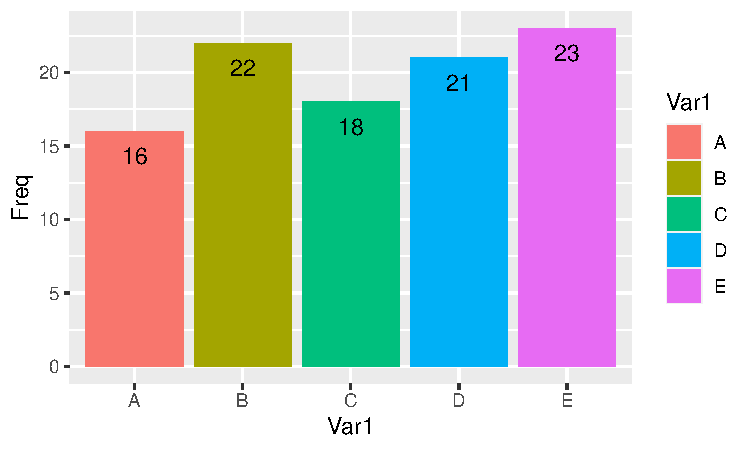
\includegraphics[width=\maxwidth]{figure/unnamed-chunk-1-1} 

}


\end{knitrout}
\end{document}
